\documentclass[12pt, titlepage]{article}

\usepackage{booktabs}
\usepackage{tabularx}
\usepackage{hyperref}
\usepackage{amssymb, amsmath}
\usepackage{enumerate}
\usepackage{mdframed}
\usepackage{color}
\usepackage{soul}
\usepackage{framed}
\usepackage{siunitx}
\usepackage{graphicx}
\usepackage{tabu}
\usepackage{multirow}
\usepackage{float} % here for H placement parameter
\usepackage{enumitem}
\usepackage{graphicx}
\graphicspath{ {./images/} }



\usepackage[round]{natbib}

%anticipated changes
\newcounter{acnum}
\newcommand{\actheacnum}{AC\theacnum}
\newcommand{\acref}[1]{AC\ref{#1}}

%unlikley chagnes
\newcounter{ucnum}
\newcommand{\uctheucnum}{UC\theucnum}
\newcommand{\uref}[1]{UC\ref{#1}}

%module ref
\newcounter{mnum}
\newcommand{\mthemnum}{M\themnum}
\newcommand{\mref}[1]{M\ref{#1}}

\title{Carbon Charts: Module Guide\\}


\author{
    McMaster University\\
    Group 18 \\ \\
    Darsi Anandarajah \\
    Justin Licari \\
    Eliad Moosavi \\
    Thomas Mullen \\
    Richard Zhang \\
}


\date{December 19, 2018}
\setcounter{tocdepth}{5}
\setcounter{secnumdepth}{5}
\begin{document}

\maketitle

\pagenumbering{roman}
\tableofcontents
\listoftables
\listoffigures
\begin{table}[bp]
\caption{\bf Revision History}
\begin{tabularx}{\textwidth}{p{3cm}p{2cm}p{4cm}p{3cm}}
\toprule {\bf Date} & {\bf Version} & {\bf Notes} & {\bf Revision}\\
\midrule
17/12/2018 & 1.0  & Created document &  REV-0 \\

\bottomrule
\end{tabularx}
\end{table}

\newpage

\pagenumbering{arabic}

\section{Introduction}

\subsection{Purpose}
This document outlines the system and component design of a data visualization library, Carbon Charts. This document will provide detailed information on the design strategies, programming principles and architectural patterns employed in the design of Carbon Charts. This document will serve as the module guide, providing module decomposition logic and the criteria used to assign responsibilities amongst major modules. Module decomposition rules are based on information hiding and described by:
\begin{itemize}
    \item The role played by the individual modules in the overall system operation.
    \item The secrets associated with each module.
    \item The facilities provided by each module. 
\end{itemize}



\subsection{Scope}
Our project is centered around creating a charting library for IBM's Carbon Design ecosytem of front-end modules, while ensuring it is accessible, reliable, performant, and feature-rich. \\
\\
\textbf{In addition to core functionality and charting types, we hope to implement:}
\begin{itemize}
    \item Bubble Charts
    \item Area charts (individual and stacked)
    \item Combo charts
\end{itemize}
\\
\textbf{In respect to accessibility, reliability, performance, we hope to implement:}
\begin{itemize}
    \item Devops and build process optimization
    \item Screen reader accessibility
    \item RTL support
    \item Zoom and scroll support
    \item Threshold support
\end{itemize}
\\
\textbf{In respect to demonstrating the library, we hope to implement:}
\begin{itemize}
    \item A micro controller with sensors feeding real time data to the library and showing it in the graphs
\end{itemize}

\subsection{Development Methods}

The project will be developed with the JavaScript environment NodeJS. Git will be used for version control using the GitHub client. Each group member will maintain their own up to date fork of the Carbon Charts library. Commits are merged in upon successful pull request.

\subsection{Assumptions}
\begin{itemize}
    \item It is assumed that developers will use library functions correctly, and pass in the correct data types within the correct data range.
\end{itemize}

\subsection{Acronyms and Definitions}
\begin{enumerate}
    \item Axis Chart: Axis charts display data between a set of axis. Axis charts are 2 or 3 dimensional, with at least an x and y axis.
    \item Non-Axis Chart: Axis charts display data within an area not defined by axis. (e.g. Pie Charts).
    \item Right-to-Left Support: The ability to display languages that read right to left, such as Farsi.
    \item Browser Tiers: We define two tiers of browsers A and B. Tier A browsers consist of the two latest versions of Chrome, Firefox, Opera and Safari at any time, and any versions below those including IE-11+ will be part of tier B.
    \item Test Data: A set of example data. This set will initially consist of a random sampling of all valid data within the expected range, but will be extended to any particular data that cause issues in the software as it develops. Requirements that involve the test data in their fit criterion will be considered unmet if any member of the test data fail that requirement.
    \item Demonstration Environment: An environment resembling a common household room; no extreme conditions (temperature, pressure, magnetic fields, impact forces etc).
    \item Internalization
\end{enumerate}

%\subsection{General Constraints}
%Darsi: What other constrains, even with D3 that puts constrains on what we can achieve.

%Carbon Charts serves as a functional component of IBM's Carbon Design System. As a result, design decisions, feature requests are subject to validation and verification via IBM's Design Team. 

%Darsi: can someone explain to me why these are constraints
%-All commits must conform to IBM's coding guidelines (formatting, coding style, etc). 
%- npm run lint

\section{Design Strategies}
Separation due to abstraction greatly reduces the complexity of software development and helps to increase the reliability of the whole system. This allows for greater flexibility in software analysis, design and development. \\
\\
\textbf{The charting library will respect these main design principles:}
\begin{enumerate}
    \item Object-Oriented Programming
        \begin{itemize}
            \item The use of object abstraction to specify and reason about different components of the software will increase readability and maintainability of the software.
            \item This is an extremely common paradigm, allowing developers to more easily contribute through open-source commits.
        \end{itemize}
    \item Encapsulation
    \begin{itemize}
        \item Modules will restrict unnecessary external access to their internal components.
        \item This reduces coupling between modules and reduces the API surface, allowing for simpler testing and reduced complexity.
        \item This is implemented using file-splitting and tooling to compile bundles (see Development Process document for more information). 
    \end{itemize}
    \item Inheritance
    \begin{itemize}
        \item All chart classes are implemented as subclasses of parent chart classes.
        \item This pattern maps the class hierarchy in design to a hierarchy in implementation and also minimizes duplication of code. \\
    \end{itemize}
\end{enumerate}


%The Carbon Charts library is designed to add new charts as sub-classes of 2 different kinds of base charts (base axis charts, which are charts with an axis, and base charts, which don't have an axis).

%These superclasses need to be considered when adding new charts to the library. If a new chart cannot be implemented as a subclass as the 2 base charts, a new superclass should be added.
\\
\textbf{General Design Principles employed by the library include:}
\begin{itemize}
    \item Principle of Low Coupling and High Cohesion 
    \item Open-Closed Principle 
    \item Liskovs Substitution Principle
    \item Dependency Inversion Principle
    \item Interface Segregation Principle
    \item Law of Demeter
\end{itemize}

\section{Anticipated and Unlikely Changes}

\subsection{Anticipated Changes}
Anticipated changes are the source of the information that is to be hidden inside the modules.
Ideally, changing one of the anticipated changes will only require changing the one module
that hides the associated decision. The approach adapted here is called design for change.

\begin{description}
\item[\refstepcounter{acnum} \actheacnum \label{acFeatureAddition}:] Modules may need to be added as it is likely that shareholders will require new chart types for different scenarios.
\item[\refstepcounter{acnum} \actheacnum \label{acFeatureRequests}:] Existing module functionality may be added, removed or modified. 
\item[\refstepcounter{acnum} \actheacnum \label{acFeatureRequests}:] Modules may need to be be added or fixes for Bug/Feature requests via stakeholders or the contributing community.
\item[\refstepcounter{acnum} \actheacnum \label{acFeatureRequests}:] New sensor hardware and types of sensors may require new modules.
\item[\refstepcounter{acnum} \actheacnum \label{acFeatureRequests}:] Combo Chart functionality will be improved.
\item[\refstepcounter{acnum} \actheacnum \label{acFeatureRequests}:] Modules may be improved for library requirements and performance.
\end{description}

\subsection{Unlikely changes}
To avoid making modification to the module, following are unlikely to change:

\begin{description}
\item[\refstepcounter{ucnum} \uctheucnum \label{ucInput}:]Carbon Design language: IBM has not ratified their design language as any kind of standard and may decide to make modifications or clarifications to it.
\item[\refstepcounter{ucnum} \uctheucnum \label{ucIO}:] Input and output devices (Input: Keyboard and mouse clicks, Output: console window)
\item[\refstepcounter{ucnum} \uctheucnum \label{ucInput}:] There will always be a source of input data external to the software.
\item[\refstepcounter{ucnum} \uctheucnum \label{ucInput}:] Individual chart functionality.
\item[\refstepcounter{ucnum} \uctheucnum \label{ucInput}:] Library requirements (open-source, interactive, lightweight and feature rich).  
\end{description}
\newpage
\section{Module Hierachy}
This section provides an overview of the module design. Modules are summarized in a hierarchy decomposed by secrets in Table \ref{TblMH}. The modules listed below, which are leaves in the hierarchy tree, are the modules that will actually be implemented.

\begin{table}[H]
\centering
\begin{tabular}{p{0.3\textwidth} p{0.6\textwidth}}
\toprule
\textbf{Level 1} & \textbf{Level 2}\\
\midrule

\multirow{16}{0.3\textwidth}{Behaviour-Hiding Module} 
& M1\\
& M2\\
& M3\\
& M4\\
& M5\\
& M6\\
& M7\\ 
& M8\\
& M9\\
& M10\\
& M11\\ 
& M12\\
& M13\\
& M14\\
& M15\\
& M16\\
\midrule

\multirow{3}{0.3\textwidth}{Software Decision Module} \\
& M17\\
& M18\\
& M19\\
& M20\\
& M21\\
& M22\\

\midrule

{Hardware-Hiding Module} & M23 \\

\bottomrule

\end{tabular}
\caption{Module Hierarchy}
\label{TblMH}
\end{table}

%\begin{table}[]
%\begin{tabular}{lllll}
%\textbf{Behaviour-Hiding Modules} & 6.1.1  & 6.1.2  & 6.1.3  & 6.1.4  \\
%\textbf{}                         & 6.1.5  & 6.1.6  & 6.1.7  & 6.1.8  \\
%                                  & 6.1.9  & 6.1.10 & 6.1.11 & 6.1.12 \\
%\textbf{}                         & 6.1.13 &        &        &        \\
%\textbf{Software Decision Module} & 6.2.1  & 6.2.2  & 6.2.3  &        \\
%\textbf{Hardware Hiding Module}   & 6.3.1  &        &        &        \\   
%\end{tabular}
%\end{table}


\section{Connection Between Requirements and Design}
The main motive of designing the system is to ensure that all the requirements in SRS document are met. Throughout the document the system is decomposed into modules and analyzed. The relation is listed in the Trace between Requirements and Modules table.

\section{Module Decomposition}

\subsection{Behavior Hiding Modules}
\begin{figure}[H]
\centering
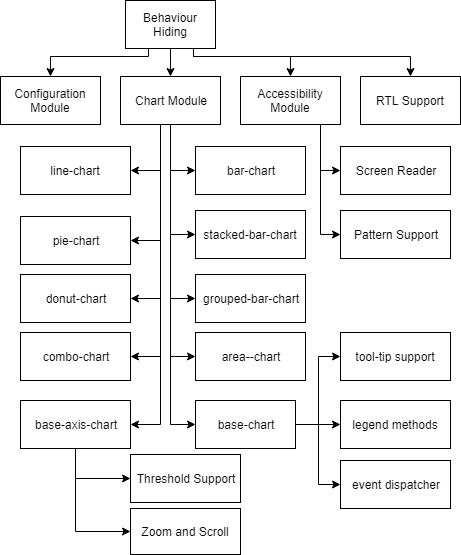
\includegraphics[width=0.7\textwidth]{behave.png}
\caption{Behaviour Hiding Module Decomposition}
\label{FigUH}
\end{figure}


\subsubsection{M1: Configuration Module}
\begin{description}[style=nextline]
\item[Type:] Configuration Module
\item[Secrets:] The style and configuration scheme used to provide configuration options to all charts. 
\item[Responsibilities:] Storing and maintaining options for chart configuration 
\item[Requirements:] No additional Requirements
%\item[Design:] Not a leaf module.
\end{description}

\subsubsection{M2: Base Chart Module}
\begin{description}[style=nextline]
\item[Type:] Chart Module
\item[Secrets:] Canvas setup, DOM interaction, tooltip functionality, and legend functionality. %Rendering, user-event handling schemes
\item[Responsibilities:] This module is responsible for providing the base functionality for all charts. Methods in Base-Chart are inherited by all charts.
\item[Requirements:] No additional Requirements
%\item[Design:] Not a leaf module
\end{description}


\subsubsection{M3: Base Axis Chart Module}
\begin{description}[style=nextline]
\item[Type:] Chart Module
\item[Secrets:] The methods used to determine how data maps to a pixel value on a Cartesian grid. 
\item[Responsibilities:] This module is responsible for calculating the scales, setting the axes and rendering data points on axes that follow a Cartesian grid. 
\item[Requirements:] No additional requirements
%\item[Design:] 
\end{description}

\paragraph{M4: Threshold Support Module}
\begin{description}[style=nextline]
\item[Type:] Base Axis Chart Module
\item[Secrets:] The methods and rules determining threshold support on base axis charts. 
\item[Responsibilities:]  This module is responsible for determining and providing threshold support to charts derived from base axis charts. 
\item[Requirements:] FN-7
\end{description}

\paragraph{M5: Zoom and Scroll Support Module}
\begin{description}[style=nextline]
\item[Type:] Base Axis Chart Module
\item[Secrets:] The methods and rules providing zoom and scroll functionality to base axis chart. 
\item[Responsibilities:]  This module is responsible for determining and providing zoom and scroll support to charts derived from base axis charts. 
\item[Requirements:] FN-8
\end{description}


\subsubsection{M6: Bar Chart Chart Module}
\begin{description}[style=nextline]
\item[Type:] Chart Module
\item[Secrets:] The methods and rules determining event-handling and how data points maps to a pixel on a bar chart.  
\item[Responsibilities:] This module is responsible for getting scale information, display data, and rendering data points on axes that follow a bar chart configuration. 
\item[Requirements:] FN-12
\end{description}


\paragraph{M7: Stacked Bar Chart Chart Module}
\begin{description}[style=nextline]
\item[Type:] Chart Module
\item[Secrets:] The methods and rules determining event-handling and how data points maps to a pixel on a stacked bar chart. 
\item[Responsibilities:]  This module is responsible for getting scale information, display data, and rendering data points on axes that follow a stacked-bar chart configuration.
\item[Requirements:] FN-13
\end{description}

\paragraph{M8: Grouped Bar Chart Chart Module}
\begin{description}[style=nextline]
\item[Type:] Chart Module
\item[Secrets:] The methods and rules determining event-handling and how data points maps to a pixel on a grouped bar chart. 
\item[Responsibilities:]  This module is responsible for getting scale information, display data, and rendering data points on axes that follow a grouped-bar chart configuration.
\item[Requirements:] FN-12
\end{description}


\subsubsection{M9: Line Chart Module}
\begin{description}[style=nextline]
\item[Type:] Chart Module
\item[Secrets:] The methods and rules determining event handling and how data points map to pixels on line charts.
\item[Responsibilities:] The module is responsible for determining scale and display data configurations as well as rendering data points on axes that follow a line-chart configuration. 
\item[Requirements:] FN-20 
\end{description}

\subsubsection{M10: Pie Chart Module}
\begin{description}[style=nextline]
\item[Type:] Chart Module
\item[Secrets:] The methods and rules determining event-handling and how data points map to pixels on pie charts.
\item[Responsibilities:] The module is responsible for determining scale, data representation, display data configurations and rendering data points on axes that follow a pie-chart configurations. 
\item[Requirements:] FN-14, FN-15, FN-16, FN-17, FN-18
\end{description}


\subsubsection{M11: Donut Chart Module}
\begin{description}[style=nextline]
\item[Type:] Chart Module
\item[Secrets:] The methods and rules determining event-handling, donut center, pie slices and how data points map to pixels on donut charts.
\item[Responsibilities:] The module is responsible for determining scale, display data configurations and rendering data points on axes that follow a donut-chart configurations.
\item[Requirements:] FN-14, FN-15, FN-16, FN-17, FN-18
\end{description}


\subsubsection{M12: Bubble Chart Module}
\begin{description}[style=nextline]
\item[Type:] Chart Module
\item[Secrets:] The methods and rules determining event-handling and how data points map to disks on bubble charts.
\item[Responsibilities:] The module is responsible for determining scale, disk size, display data configurations and rendering data points on axes that follow a bubble-chart configuration options. 
\item[Requirements:] FN-14, FN-15, FN-19
\end{description}

\subsubsection{M13: Area Chart Module}
\begin{description}[style=nextline]
\item[Type:] Chart Module
\item[Secrets:] The methods and rules determining event-handling and how data points map to area segments between the x-ais.
\item[Responsibilities:] The module is responsible for determining scale, area functions, display data configurations and rendering data points on axes that follow a area-chart configuration options.
\item[Requirements:] FN-21
\end{description}

\subsubsection{M14: Combo Chart Module}
\begin{description}[style=nextline]
\item[Secrets:] The methods and rules determining event-handling and how different chart types are displayed on a common axis-chart.
\item[Responsibilities:] The module is responsible for determining the scale, tool-tip options, representation of data points by chart type, positioning of charts and rendering multiple charts on a common base-axis chart.
\item[Requirements:] No addional requirements. 
\end{description}

\subsubsection{M15: Screen Reader Accessibility Module}
\begin{description}[style=nextline]
\item[Type:] Accessibility  Module
\item[Secrets:] Methods providing accessibility support to supported chart types.
\item[Responsibilities:] This module is responsible for providing accessibility support via screen reader services for charts. 
\item[Requirements:] Usability-req-1
\end{description}

\subsubsection{M16: RTL Support Module}
\begin{description}[style=nextline]
\item[Type:]  RTL Support Module
\item[Secrets:] Rules and methods determining how right-to-left support is used in chart rendering.
\item[Responsibilities:]  This module is responsible for providing RTL support for charts. 
\item[Requirements:] Compliance-req-1
\end{description}


\subsection{Software Decision Hiding Modules}
\begin{figure}[H]
\centering
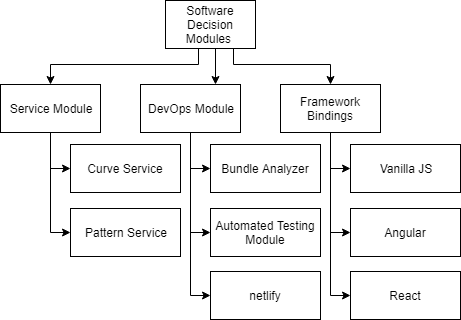
\includegraphics[width=0.7\textwidth]{software-decision-decomp.png}
\caption{Software Decision Hiding Module Decomposition}
\label{FigUH}
\end{figure}

\subsubsection{M17: Pattern Service Module}
\begin{description}
\item[Type:] Service Module
\item[Secrets:] The methods used to provide accessibility support via patterns.     
\item[Responsibilities:] Responsible for providing the pattern service to base-charts inherited by all charts. 
\item[Requirements:] Usability-req-2
\end{description}


\subsubsection{M18: Curve Service Module}
\begin{description}
\item[Type:] Service Module
\item[Secrets:] D3 curve functionality for line generators. 
\item[Responsibilities:] This module is responsible for providing D3 curve service for line and combo charts.
\item[Requirements:] FN-20
\end{description}

\subsubsection{M19: Bundle Analyzer Module}
\begin{description}
\item[Type:] DevOps Module
\item[Secrets:] The methods used to determine bundle size of the library.  
\item[Responsibilities:]  This module is a devOps tool responsible for calculating and reporting the bundle size of the library. 
\item[Requirements:] PERF-1
\end{description}


\subsubsection{M20: Automated Testing Module}
\begin{description}[style=nextline]
\item[Type:]  DevOps Module
\item[Secrets:] Rules and test cases ensuring correctness of chart functionality.
\item[Responsibilities:]  This module is responsible for providing test cases to verify and validate chart functionality. 
\item[Requirements:] No additional Requirements
\end{description}

\subsubsection{M21: Netlify Module}
\begin{description}[style=nextline]
\item[Type:]  DevOps Module
\item[Secrets:] Pull request verification and validation.  
\item[Responsibilities:]  This module is responsible for providing a means of verifying and validating to repository managers. 
\item[Requirements:] No additional Requirements
\end{description}

\subsubsection{M22: Framework Bindings Module}
\begin{description} [style=nextline]
\item[Type:] Framework Module
\item[Secrets:] The supported frameworks and rules determining framework bindings. 
\item[Responsibilities:]  This module is responsible for framework support, bindings and framework specific configuration options. Additionally, it determines how model updating, rendering, event-handling and user interaction is bound to the framework.
\item[Requirements:] No additional requirements. 
\end{description}

\newpage
\subsection{Hardware Hiding Modules}
\subsubsection{M23: Communication Module}
\begin{description}[style=nextline]
\item[Type:] Onboard Module
\item[Secrets:] The methods and protocol used to communicate with the hardware component.
    \item How incoming data is serialized into JSON objects that are consumable by the charting library.
    \item Chart configuration and event listeners that are specific to the hardware sensor array demonstration.
\item[Responsibilities:] Abstracting implementation specifics of the hardware sensor array and it's communication channel.
\item[Requirements:] FN-22, FN-23
\end{description}

\newpage
\section{Module Designs}
\subsection{Module Interface Specification}

\href{https://carbon-design-system.github.io/carbon-charts/documentation/}{Documentation publicly available.}
\subsection{Base Chart Module}
The Base Chart implements the core charting and rendering functionality that is inherited by all other chart types. This includes canvas setup, DOM interaction, tooltip functionality, and legend functionality. It is an abstract class and cannot be directly instantiated.
%This module serves as the super class of all charts. Every chart is inherently derived from base-chart.

\subsubsection{Interface}
\begin{table}[H]
\begin{tabular}{llp{6cm}}
\textbf{Uses}            & Configuration Module     &                                                                      \\
\textbf{Constants}       & None                     &                                                                      \\
\textbf{Types}           & None                     &                                                                      \\
\textbf{Access Programs} & getKeysFromData         & Builds key and returns key array for legend item objects.\\            \\
                         & getLegendType            & Returns legend type for chart from configuration module              \\\\
                         & getChartSize             & Returns chart size based on chart container and clientWidth property \\ \\
                         & updateSVG                & Updates svg element \\                                                                     \\
                         & getLegendItems           & Returns legend items \\                                                                     \\
                         & addTooltipEventListeners &                                                                      \\
                         & getFillScale             &                                                                      \\
                         & getDefaultTransition     &                                                                      \\
                         & getInstantTransition     &                                                                      \\
                         & getFillTransition        &                                                                      \\
                         & getBBox                  &                                                                     
\end{tabular}
\end{table}

\subsection{Base Axis Chart Module}
The Base Axis Chart extends the Base Chart, adding axis functionality, zoom/scroll control, and chart scaling. It is an abstract class and cannot be directly instantiated.
% Please add the following required packages to your document preamble:
% \usepackage{multirow}
\begin{table}[H]
\begin{tabular}{l p{5cm}p{5cm}}
\textbf{Uses}            & None                                   &                                                     \\
\textbf{Constants}       & None                                   &                                       \\
\textbf{Types}           & None                                   &                                                     \\
\textbf{Access Programs} & initialDraw(data?: any)                & Called when the chart needs to be drawn initially.  \\
                         & update()                               & Populate display data, sets x and y axis and scale. \\
                         & addLabelsToDataPoints(d, index)        & Adds labels to data points based on display data.   \\
                         & getChartSize(container)                & Returns height and width of chart size.             \\
                         & resizeChart()                          & Repositions legend , axis-labels and scale.         \\
                         & setXScale (xScale?: any)                & Scales x-axis, labels and margins.                  \\
\textbf{}                & setXAxis(noAnimation?: boolean)        & Sets x-axis, labels and margins.                    \\
                         & setYScale (xScale?:any)                 & Scales y-axis, labels and margins.                  \\
                         & setYAxis(noAnimation?: boolean)         & Scales y-axis, labels and margins.                  \\
                         & updateXandYGrid (noAnimation? : boolean) & Updates x and y grid upon event. \\                    
\end{tabular}
\end{table}


\newpage
\subsection{Bar Chart Module}
The Base Chart extends the base-axis-chart, adding functionality for bar and stacked-bar rendering functionality and data point labeling.
\subsubsection{Interface}
\begin{table}[H]
\begin{tabular}{l p{5cm}p{5cm}}
\textbf{Uses}            & Base-Axis-Chart Module                     &                                                                                                                  \\
\textbf{Constants}       & None                                     &                 \\
\textbf{Types}           & None                                       &                                                                                                                  \\
\textbf{Access Programs} & constructor(holder:Element, configs: any) & bar-chart constructor                                                                                            \\
                         & draw()                                     & Render bar-chart                                                                                                 \\
                         & interpolateValues(newData: any)            & Creates/Update bar chart: add bars to chart, respond to events via addDataPointEventListener and dispatchEvent() \\
                         & addDataPointEventListener()                & Adds toop-tip functionality specific to bar charts                                                               \\
                         & resizeChart()                              & Repositions legend, axis-labels and scale.\\                                                                     
\end{tabular}
\end{table}




%\subsubsection{State Variables}
%\subsubsection{Access Routines}
% TODO: Correctness? Consistency?
\newpage
\subsection{Line Chart}
The Line Chart extends the Base Axis Chart, adding line/curve rendering functionality, line animation, and data point labeling. 
\subsubsection{Interface}
\begin{table}[H]
\begin{tabular}{l p{5cm}p{5cm}}
\textbf{Uses}            & Base-Axis-Chart Module                     &                                                                                                                  \\
\textbf{Constants}       & None                             &                                                                                                     \\
                         
\textbf{Types}           & None                                       &                                                                                                                  \\
\textbf{Access Programs} & constructor(holder: Element, configs: any) & line-chart constructor                                                                                            \\
                         & draw()                                     & Render line-chart                                                                                                 \\
                         & interpolateValues(newData: any)            & Creates/Update line chart: add lines to chart, respond to events via addDataPointEventListener and dispatchEvent() \\
                         & addDataPointEventListener()                & Adds toop-tip functionality specific to lines charts                                                               \\
                         & resizeChart()                              & Repositions legend, axis-labels and scale.\\                                                                     
\end{tabular}
\end{table}


\newpage
\subsection{Pie Chart}
The Pie Chart extends the Base Chart, adding functionality to render circular charts and additional data processing to translate data into proportions. 

\begin{table}[H]
\begin{tabular}{l p{5cm}p{5cm}}
\textbf{Uses}            & Base-Chart Module                     &                                                                                                                  \\
\textbf{Constants}       & None                             &                                                                                                     \\
                         
\textbf{Types}           & None                                       &                                                                                                                  \\
\textbf{Access Programs} & constructor(holder: Element, configs: any, type: string) & pie-chart constructor                                                                                            \\
                         & dataProcessor(dataObject: any)             & Prepares data for pie chart rendering. \\
                         & draw()                                     & Render pie-chart                                                                                                 \\
                         & interpolateValues(newData: any)            & Creates/Update pie chart: adds pie slices to chart, interpolates transitions, responds to events via addDataPointEventListener and dispatchEvent() \\
                         & addDataPointEventListener()                & Adds toop-tip functionality specific to pie charts                                                               \\
                         & resizeChart()                              & Repositions legend, pie segments and scale.\\  
\end{tabular}
\end{table}

\newpage
\subsection{Donut Chart}
The Donut Chart extends the Pie Chart. It is exclusively a stylistic change, removing the center of the Pie Chart.

\begin{table}[H]
\begin{tabular}{l p{5cm}p{5cm}}
\textbf{Uses}            & Pie-Chart Module                     &                                                                                                                  \\
\textbf{Constants}       & None                             &                                                                                                     \\
                         
\textbf{Types}           & None                                       &                                                                                                                  \\
\textbf{Access Programs} & constructor(holder: Element, configs: any, type: string) & Donut chart constructor                                                                                            \\
                         & draw()                                     & Render donut-chart  \\
                         & Update(newData: any)                       & Update donut chart if configs are different from previous update call.
                         & addDataPointEventListener()                & Adds toop-tip functionality specific to pie charts                                                               \\
                         & resizeChart()                              & Inherits resizing logic from PieChart, superclass class is encapsulated in function.\\  
\end{tabular}
\end{table}


% TODO: Other chart types (do the above first)
\newpage
\subsection{Pattern Service}
The pattern service is used for the accessibility mode on all charting components. It is in charge of parsing and cleaning SVG pattern files provided to it, and injecting them into the DOM. Then it will provide an array of SVG URLs for each charting component to use.
\subsubsection{Interface}
\begin{table}[H]
\begin{tabular}{l p{5cm}p{5cm}}
\textbf{Uses}            & None                     &                                                                                                                  \\
\textbf{Constants}       & PATTERNS\_CONTAINER:string                             &                                                                                                     \\
                         
\textbf{Types}           & None                                       &                                                                                                                  \\
\textbf{Access Programs} & constructor(holder:Element, configs: any, type: string) & Donut chart constructor                                                                                            \\\\
                         & addPatternSVGs (d:any, colorScale:any, chartContainerID:string, legendType:string)                                     & Adds all the pattern SVGs to the container div, applying a unique ID to each one.  \\\\
                         & getFillValues()                       & getFillValues() \\
\end{tabular}
\end{table}

\subsection{Curve Service}
This module provides D3 shape generator services. It only loads those related to supported chart types maintaining the light weight property of the library.  
\subsubsection{Interface}
\begin{table}[H]
\begin{tabular}{l p{5cm}p{5cm}}
\textbf{Uses}            & None                     &                                                                                                                  \\
\textbf{Constants}       & curveTypes[] :d3-shape                            &                                                                                                     \\
                         
\textbf{Types}           & None                                       &                                                                                                                  \\
\textbf{Access Programs} & getD3Curve(curveName: any) & Return curve generators from d3-shape library.                                                                                             \\
\end{tabular}
\end{table}

\newpage
\subsection{Hardware Component} 
\subsubsection{Purpose}
Acquire data from sensors using an Arduino Uno and other pieces of hardware. The data will then be graphically displayed by the charts in real time. Please note every sensor uses pints 5V Vcc and ground.
\subsubsection{Components}
\begin{itemize}
    \item Arduino UNO
    \item Breadboard
    \item Jumper Wires
    \item Resistors
    \item Ultrasonic Sensor
    \item Temperature Sensor
    \item Big Sound sensor
\end{itemize}
\textbf{Ultrasonic Sensor}\\ 
Detects the presence of a target object and measures the distance between the sensor and the object by sending a beam of ultrasound that is reflected off the object. Relevant pins: 
\begin{itemize}
    \item Trig (input): signal from Arduino to generate the ultrasound
    \item Echo (output): time in microseconds the sound wave travelled. Time is proportional to range of the signal. The time will be multiplied by the speed of sound to calculate distance in centimetres.
\end{itemize}
\textbf{Temperature sensor}  \\
Provides temperature measurement through an electrical signal pin:
\begin{itemize}
    \item Output pin: analog voltage reading between 0 and 1.75V. 
\end{itemize}
To convert the 10-bit analog reading into voltage: \\
Voltage at pin in millivolts = (reading from ADC) * (5000/1024) \\
Then, to convert the voltage into centigrade temperature: 
Centigrade temperature = [(analog voltage in mV) - 500]/10 \\ \\
\textbf{Big Sound Sensor} \\
Sensor that detects sound intensity by converting air pressure vibrations into electrical signals. Three pins include:
\begin{itemize}
    \item Digital output voltage: signal is proportional to sound intensity
\end{itemize}

\subsubsection{Normal operation}
Sensors will log data points using serial connection into a JSON file. This file will be opened and parsed to extract the data and display it graphically using the charting library. 

\subsubsection{Context Diagram}
\begin{figure}[h]
\centering
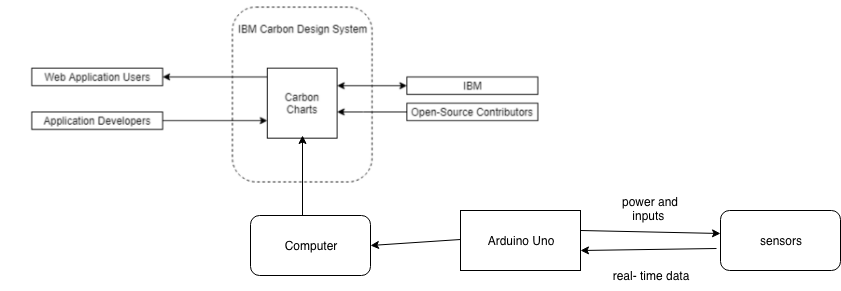
\includegraphics[width=1\textwidth]{contextDiagram.png}
\caption{Context Diagram with Hardware Interfacing Component.}
\label{FigUH}
\end{figure}

\newpage
\section{Traceability Matrix}
This section shows two traceability matrices: between the modules and the requirements and between the modules and the anticipated changes.

% the table should use mref, the requirements should be named, use something
% like fref
\begin{table}[H]
\centering
\begin{tabular}{p{0.2\textwidth} p{0.6\textwidth}}
\toprule
\textbf{Req.} & \textbf{Modules}\\
\midrule
FN-1 & M1, M2, M3\\
FN-2 & M1, M2, M3\\
FN-3 & M1, M2\\
FN-4 & M2, M3\\
FN-5 & M2 \\
FN-6 & M16\\
FN-7 & M3\\
FN-8 & M2\\
FN-9 & M1\\
FN-10 & M1, M2 \\
FN-11 & M2\\
FN-12 & M6, M7, M8\\
FN-13 & M7\\
FN-14 & M10\\
FN-15 & M11\\
FN-16 & M10, M11\\
FN-17 & M10, M11\\
FN-18 & M10, M11\\
FN-19 & M12\\
FN-20 & M9\\
FN-21 & M13\\
FN-22 & M23\\
FN-23 & M23\\
USB-1 & M15\\
USB-2 & M17\\
\bottomrule
\end{tabular}
\caption{Trace Between Requirements and Modules}
\label{TblRT}
\end{table}


\begin{table}[H]
\centering
\begin{tabular}{p{0.2\textwidth} p{0.6\textwidth}}
\toprule
\textbf{AC} & \textbf{Modules}\\
\midrule
AC1 & M1, M2 M3\\
AC2 & M2, M3\\
AC3 & M20, M21 and which ever chart/feature module is being fixed.\\
AC4 & M23 \\
AC5 & M14 \\

\bottomrule
\end{tabular}
\caption{Trace Between Anticipated Changes and Modules}
\label{TblACT}
\end{table}


\newpage
\section{Use Hierarchy Between Modules} \label{SecUse}

\begin{figure}[H]
\centering
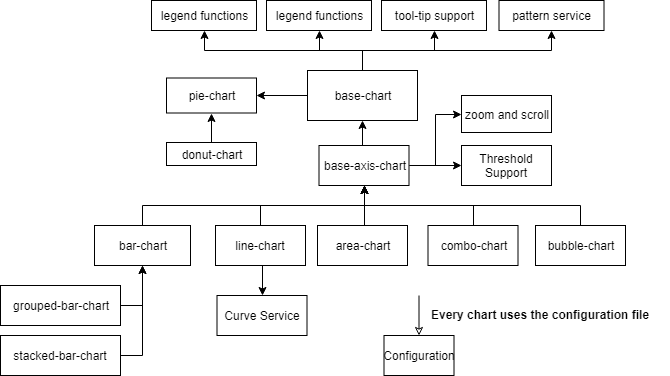
\includegraphics[width=1\textwidth]{uses-hier.png}
\caption{Hierarchy among modules}
\label{FigUH}
\end{figure}

\newpage
\section{References}
\begin{enumerate}
    \item Parnas, D.L. "Designing Software for Ease of Extension and Contraction", Proceedings of the Third International Conference on Software Engineering, pp. 264-277, 10-12 May, l978.
    \item Parnas, D.L., Paul, C.C., David, M.W. "The Modular Structure of Complex Systems", IEEE TRANSACTIONS ON SOFTWARE ENGINEERING,VOL. SE-1 1, NO. 3, MARCH 1985
    \item  Parnas, D.L., Britton, K.H. "A Procedure for designing abstract interfaces for device interface modules.", ICSE '81 Proceedings of the 5th international conference on Software engineering, pp. 195-204, 09 - 12 March, 1981. 
\end{enumerate}

\end{document}
